\chapter{Introducción}
Desde el principio de los tiempos, el ser humano se ha comunicado con sus congéneres de distintas maneras: comenzó a través de la voz (se cree que hace unos 100.000 años), con algún tipo de protolenguaje, para posteriormente comenzar a utilizar sistemas de comunicaciones permanentes (la escritura).

Algunos ejemplos a lo largo de la historia de distintos sistemas escritos son:
\begin{itemize}
    \item \textbf{Pinturas rupestres}: Realizadas en cuevas o rocas en las que se pueden observar escenas de caza, distintos animales, grabado de manos, figuras humanas... Algunas de las pinturas encontradas cuentan con más de 50.000 años. Tenemos un ejemplo cercano en las \href{https://es.wikipedia.org/wiki/Cueva_de_Santimami\%C3\%B1e}{cuevas de Santimamiñe} en donde tenemos pinturas datadas entre 14.000 y 9.000 años a. C.

    \item \textbf{Escritura jeroglífica y el papiro}: En el antiguo Egipto se crea la escritura mediante signos que comienza por escribirse en paredes para posteriormente inventar el papiro (cuya datación más antigua es del 2.500 a.C.) y de esta manera se comienza a tener un sistema de comunicación fácilmente manejable e intercambiable.

    \item \textbf{Imprenta}: El primer documento impreso data de china del año 868, pero la imprenta moderna la creó en 1440, más o menos, \href{https://es.wikipedia.org/wiki/Johannes_Gutenberg}{Johannes Gutemberg}. Gracias a la imprenta la creación de documentos escritos se realizaba de manera más rápida y esto permitió que la expansión del conocimiento escrito se acelerase.

    \item \textbf{Máquina de escribir}: Desde la invención de la imprenta, hubo distintos inventos (con distintas formas) tratando de buscar la creación de un sistema que permitiese escribir a través de un sistema mecánico. El primer sistema comercial de máquinas de escribir empezó en 1874, pero no se empezó a popularizar hasta 1880.
\end{itemize}

\section{¿Qué vamos a aprender?}


\begin{itemize}
    \item
\end{itemize}


\chapter{Edición de texto}

\section{Introducción}
Desde la invención de los ordenadores, uno de los primeros programas que se crearon fue los editores de texto: sistemas que nos permiten escribir documentos, guardarlos e imprimirlos para su posterior lectura fuera del ordenador.

Estos editores son la evolución de las máquinas de escribir, pero nos permite tener muchas más opciones que las máquinas de escribir carecían, como por ejemplo:

\begin{itemize}
    \item \textbf{Borrar texto}: en las máquinas de escribir no se podía borrar texto, sólo en los últimos modelos, que ya eran eléctricos.
    \item \textbf{Tamaño de letra}: no se podía cambiar el tamaño de letra.
    \item \textbf{Tipos de letra}: las máquinas de escribir sólo tenían un único tipo de letra.
    \item ...
\end{itemize}

Hoy día, a la hora de editar textos existen distintos tipos de programas, y vamos explicar los más habituales

\section{Sistemas de edición de texto}
A la hora de editar texto en un ordenador podemos diferenciar entre los siguientes sistemas:

\begin{itemize}
    \item \textbf{Editor de texto plano}: Es un programa que sólo nos permite una edición simplificada de texto. Sólo podemos modificar cómo el programa representa el texto, pero el fichero guardado sólo contiene el texto, nada más.

    \begin{center}
        \vspace{-10pt}
        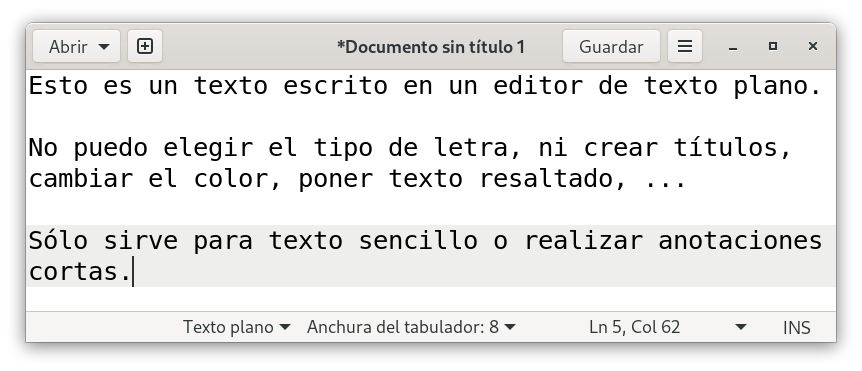
\includegraphics[width=0.6\linewidth]{editor_texto_plano.png}
        \vspace{-10pt}
    \end{center}

    \item \textbf{Procesador de texto}: Son programas que nos permiten crear documentos con formato (tipos de letra distintos, tamaños de letra, colores, imágenes,...).
    \begin{itemize}
        \item \textbf{WYSIWYG}: Del inglés “\textit{What You See Is What You Get}” (lo que ves es lo que obtienes), son los procesadores de texto más habituales en el uso diario. Estos sistemas nos permite ver cómo va a quedar el documento final a la vez que lo vamos escribiendo y/o maquetando.

        \begin{center}
            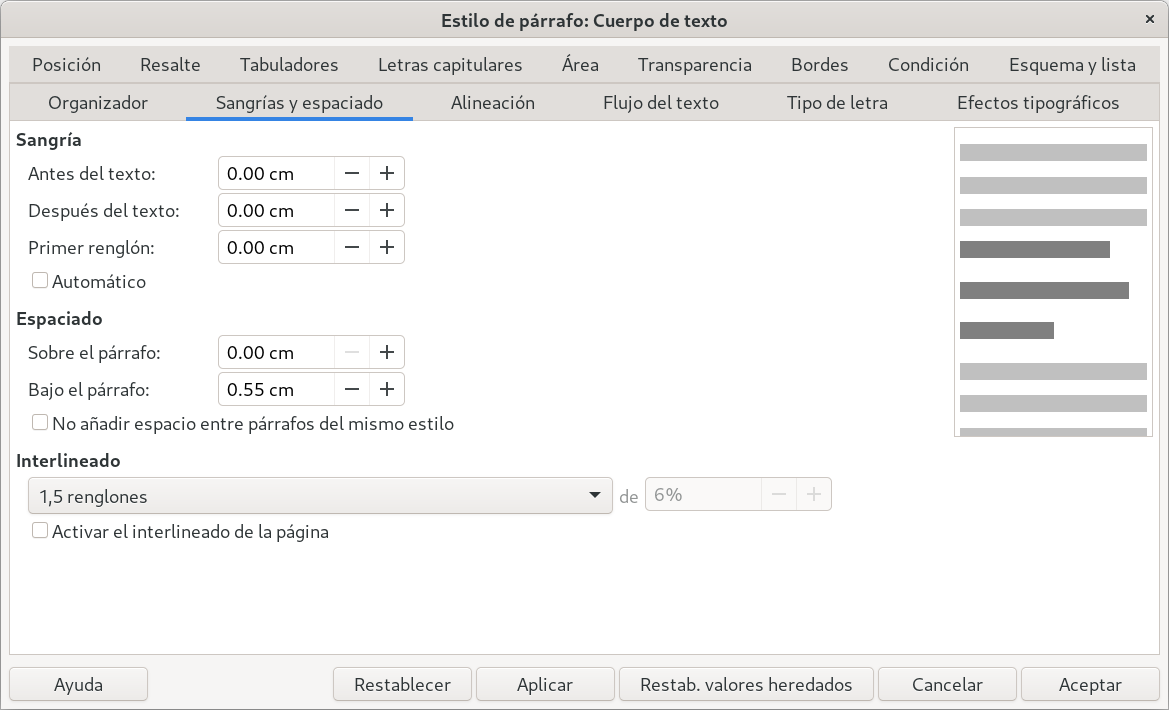
\includegraphics[width=0.6\linewidth]{libreoffice.png}
            \vspace{-5pt}
            \captionof{figure}{Editor \textbf{WYSIWYG} LibreOffice.}
            \vspace{-10pt}
        \end{center}

        \item \textbf{Texto interpretado}: Este tipo de editores permiten la escritura en texto plano del documento que posteriormente es procesado para obtener el resultado final.

        \begin{center}
            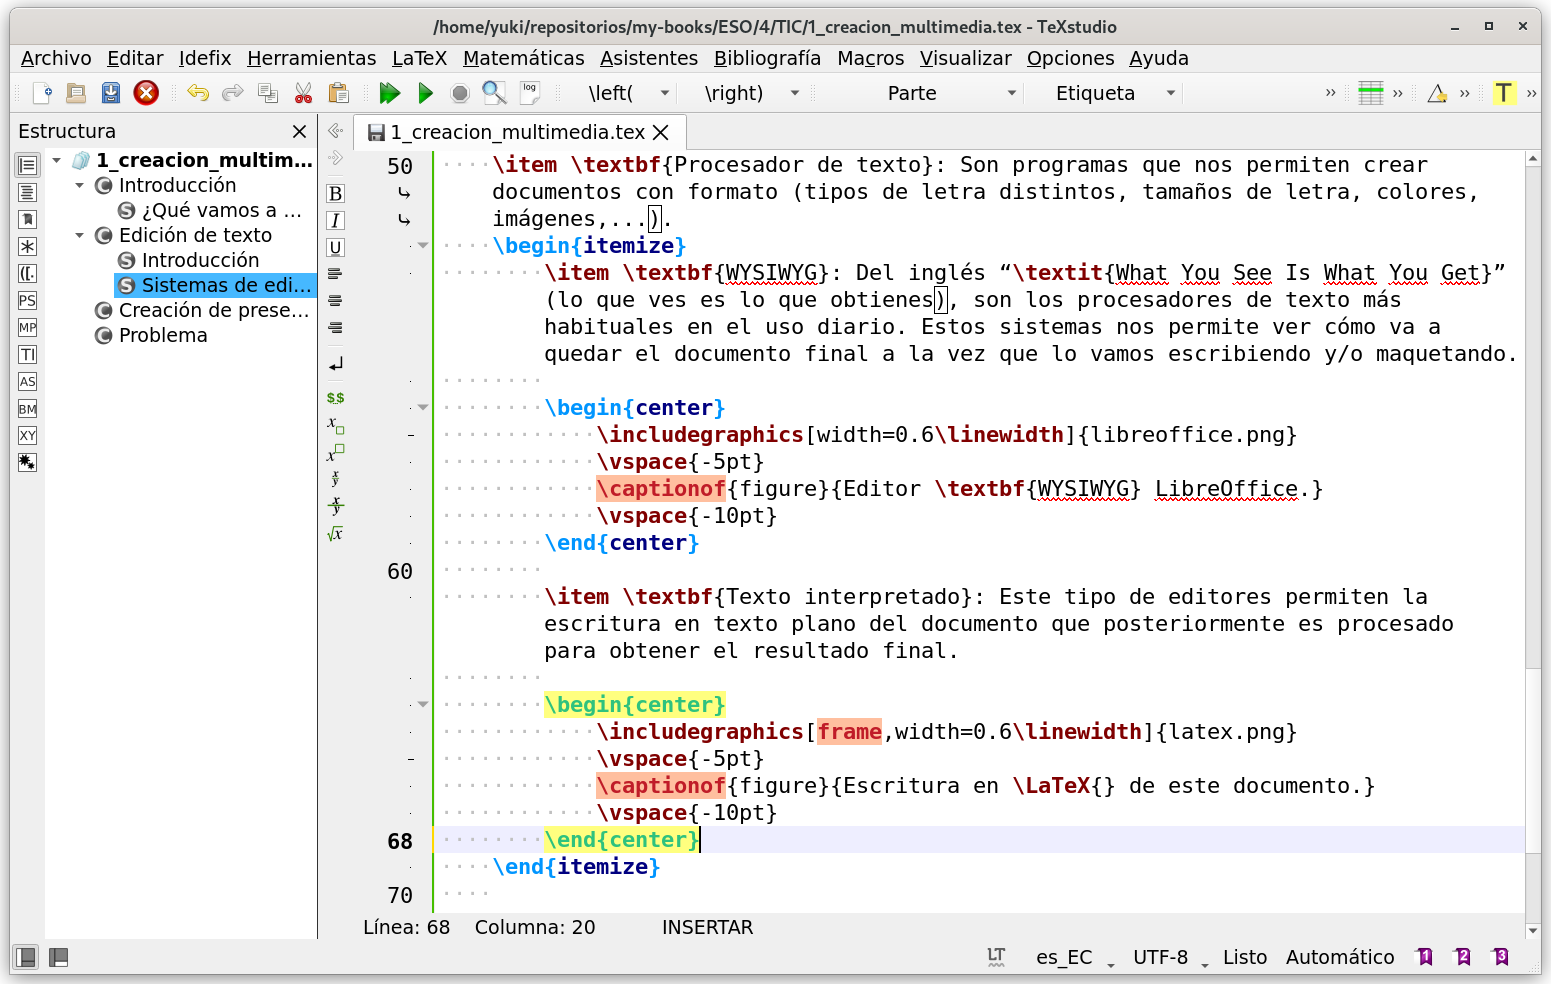
\includegraphics[width=0.6\linewidth]{latex.png}
            \vspace{-5pt}
            \captionof{figure}{Escritura en \LaTeX{} de este documento.}
            \vspace{-10pt}
        \end{center}
    \end{itemize}

\end{itemize}

\begin{tcolorbox}[title=Ejercicio,]
    Busca al menos 3 procesadores de texto \textbf{WYSIWYG} y añade la página web oficial de cada uno de ellos
    \tcblower
    \begin{itemize}
        \item
        \item
        \item
    \end{itemize}
\end{tcolorbox}


\section{Funcionalidades básicas en procesadores de texto}

\subsection{Maquetación de párrafos}

Sangría

Interlineado

Separación entre párrafos


\subsection{Títulos en los documentos}

\subsection{Índice en los documentos}


\section{Trabajando con imágenes}


\chapter{Creación de presentaciones}



\chapter{Problema}